\chapter{Interrogazione dell'ontologia}

\section{SWRL}
Sono state utilizzate regole SWRL per consentire al reasoner di inferire ulteriori informazioni sull'ontologia, in particolare riguardo al valore di energia che una batteria può assorbire o immettere.

Le regole SWRL implementate affrontano diverse casistiche e consentono al reasoner di dedurre il valore di energia in modo più accurato. In totale, sono state create quattro regole per gestire i calcoli correlati.


Per leggibilità sono stati inseriti gli screenshot delle regole, la versione testuale è disponibile nel file \href{https://github.com/19eddie/SemanticWeb-Assignment02-03/blob/main/SWRL%20energia%20che%20pu%C3%B2%20realmente%20assorbire%20o%20fornire%20una%20batteria.txt}{\textit{SWRL energia che può realmente assorbire o fornire una batteria.txt}
} reperibile sulla repository di \href{https://github.com/19eddie/SemanticWeb-Assignment02-03}{Github}. \\

\subsubsection{Premessa terminologia}
Con \textit{potenza massima di carica} (nelle regole \texttt{maxChargingPower}) si intende la massima quantità di energia elettrica che la batteria può assorbire per aumentare il suo livello di carica,
mentre con \textit{potenza massima di scarica} (nelle regole \texttt{maxDischargingPower}) si intende la massima quantità di energia elettrica che la batteria può fornire quando viene utilizzata per alimentare dispositivi o sistemi elettrici.

Invece, la \textit{capacità di carica} (nelle regole \texttt{battChargingCapacity}) di una batteria rappresenta la massima quantità di energia elettrica che può essere immagazzinata nella batteria quando viene caricata.
Mentre la \textit{capacità di scarica} (nelle regole \texttt{battDischargingCapacity}) di una batteria rappresenta la massima quantità di energia elettrica che la batteria può fornire durante il processo di scarica.


\subsection{Energia potenzialmente assorbibile = potenza massima di carica e Energia potenzialmente fornibile = potenza massima di scarica}
[\ref*{fig:bothlessorequal}] In questo caso la batteria può assorbire al massimo la potenza massima di carica siccome è inferiore o uguale alla capacità di carica,
e può fornire al più la potenza massima di scarica, perchè inferiore o uguale della capacità di scarica.

\begin{figure}[H]
    \centering
    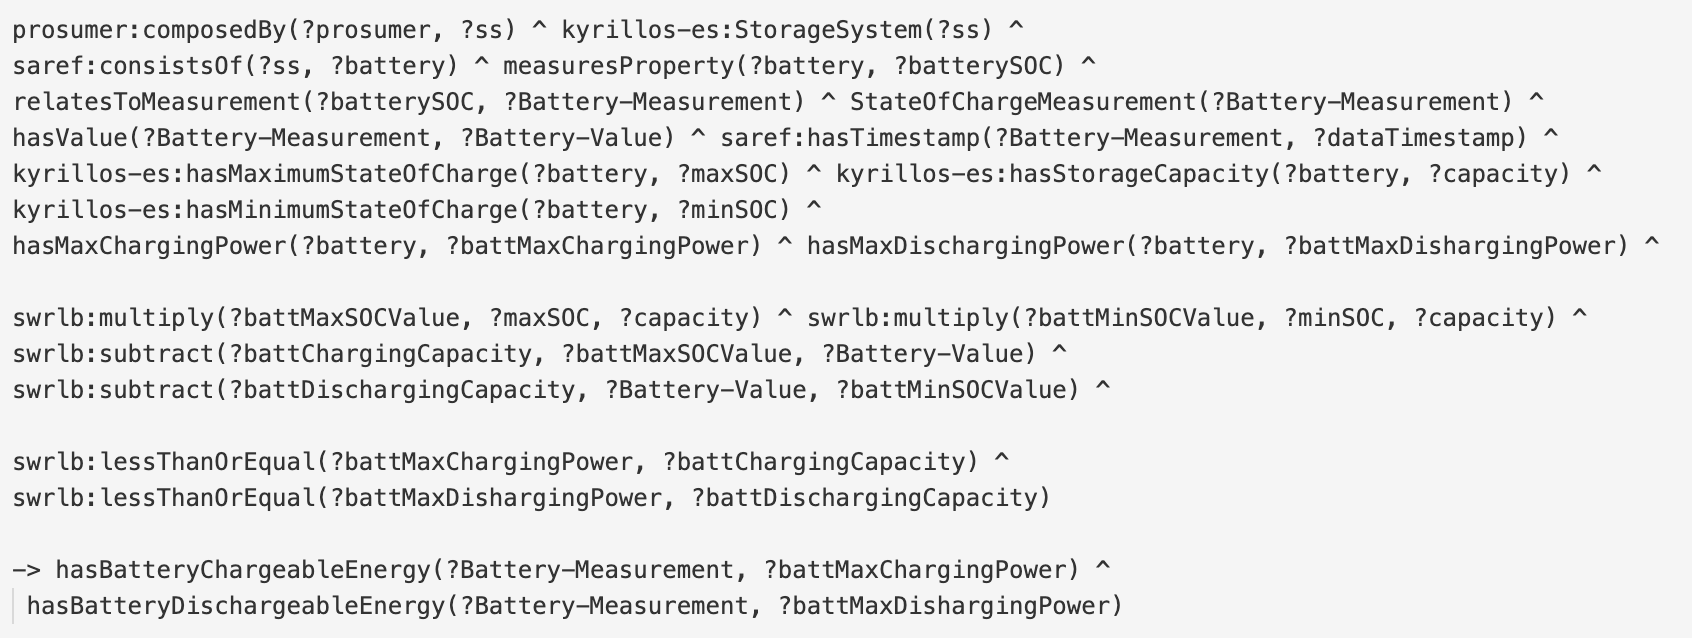
\includegraphics[width=15cm]{images/both <=.png}
    \caption{Screenshot della prima regola.}
    \label{fig:bothlessorequal}
\end{figure}


\subsection{Energia potenzialmente assorbibile = potenza massima di carica e Energia potenzialmente fornibile = capacità di scarica}
[\ref*{fig:charginglessorequal}]  Anche in questo caso la batteria può assorbire al massimo la potenza massima di carica siccome è inferiore o uguale alla capacità di carica,
e invece può fornire al più la capacità di scarica, perchè la potenza di scarica risulta maggiore della capacità.


\begin{figure}[H]
    \centering
    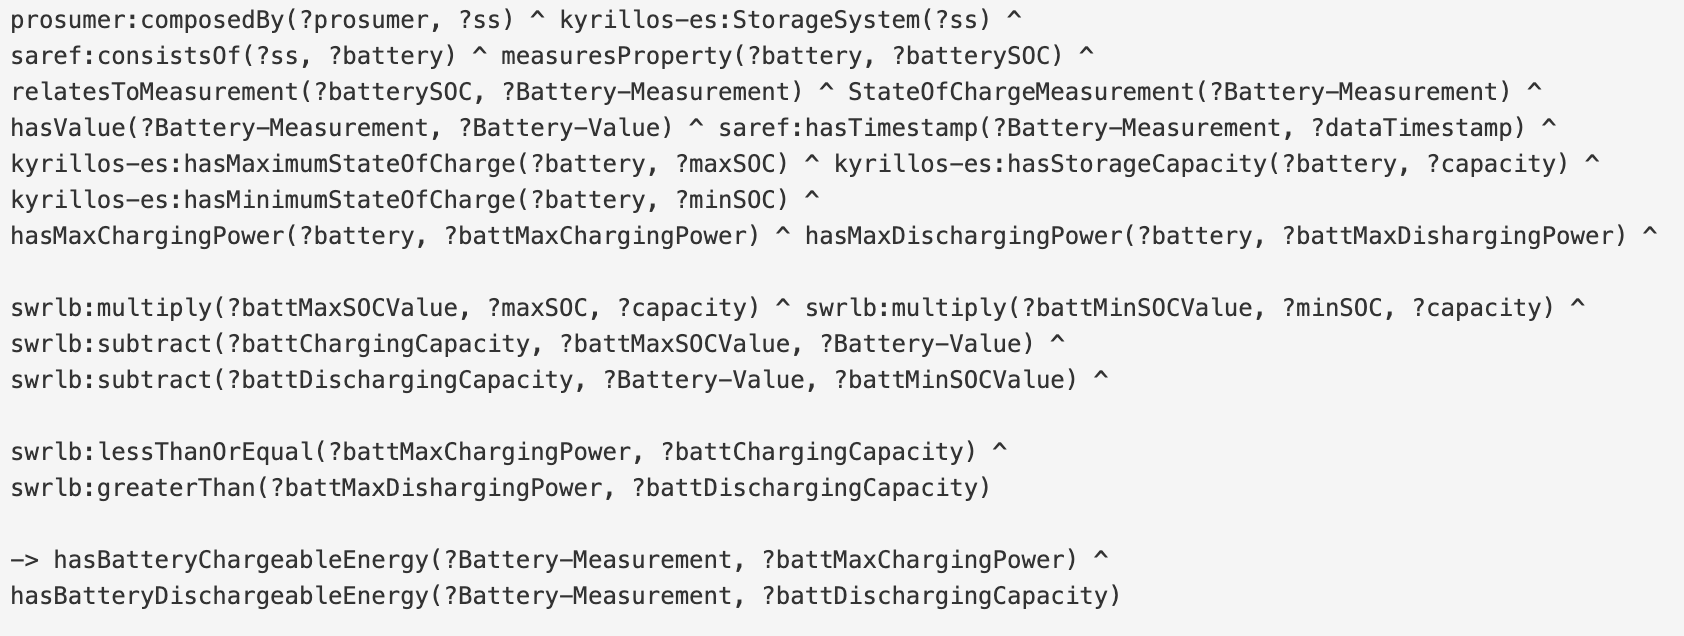
\includegraphics[width=15cm]{images/charging <=.png}
    \caption{Screenshot della seconda regola.}
    \label{fig:charginglessorequal}
\end{figure}


\subsection{Energia potenzialmente assorbibile = capacità di carica e Energia potenzialmente fornibile = potenza massima di scarica}

[\ref*{fig:charginggreater}] In questo caso invece, la capacità di carica è inferiore alla potenza massima, dunque la batteria può assorbibile al massimo la capacità di carica,
mentre può fornire al più la potenza massima di scarica, perchè inferiore o uguale alla capacità di scarica.

\begin{figure}[H]
    \centering
    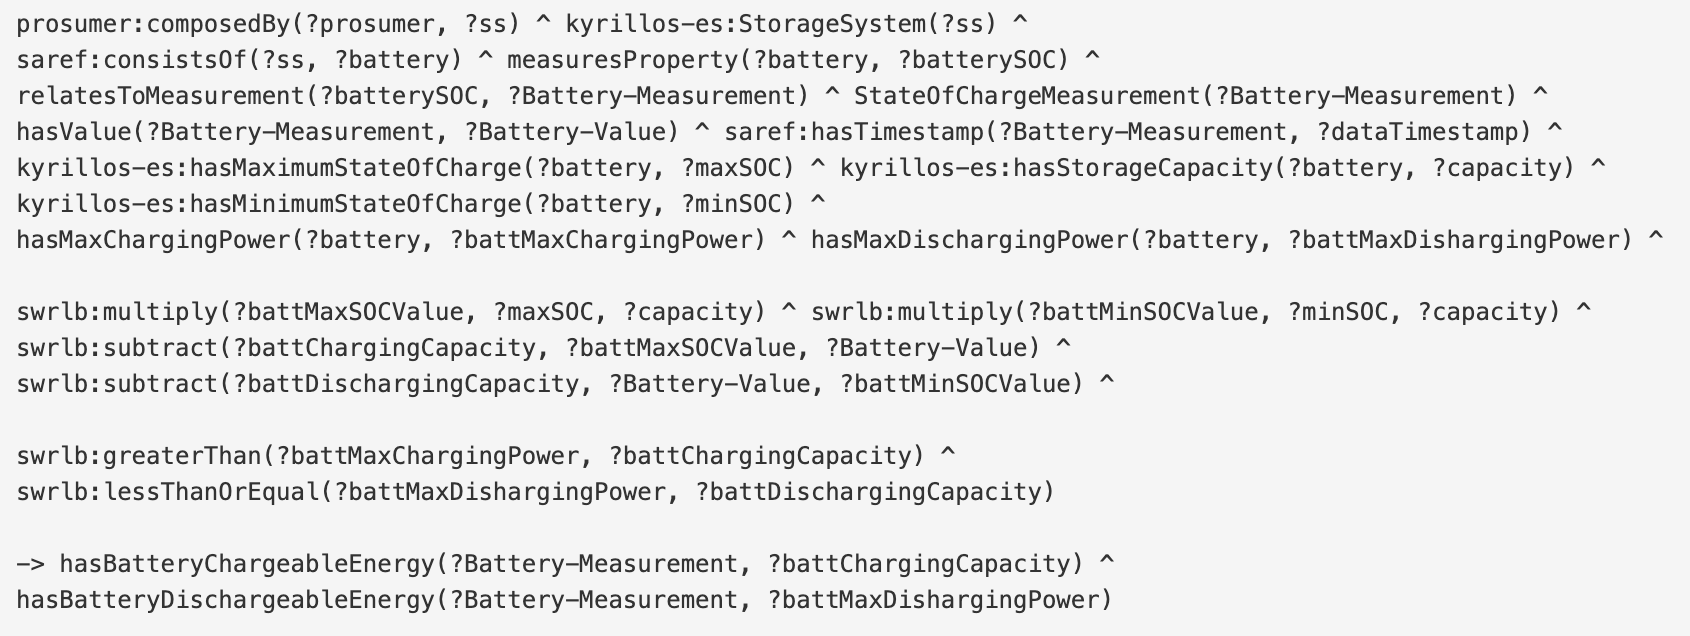
\includegraphics[width=15cm]{images/charging >.png}
    \caption{Screenshot della terza regola.}
    \label{fig:charginggreater}
\end{figure}

\subsection{Energia potenzialmente assorbibile = capacità di carica e Energia potenzialmente fornibile = capacità di scarica}

[\ref*{fig:bothgreater}] Infine c'è il caso in cui la potenza massima sia di carica che di scarica, siano superiori alle rispettive capacità che diventano dunque i valori massimi assorbibili o fornibili dalla batteria.

\begin{figure}[H]
    \centering
    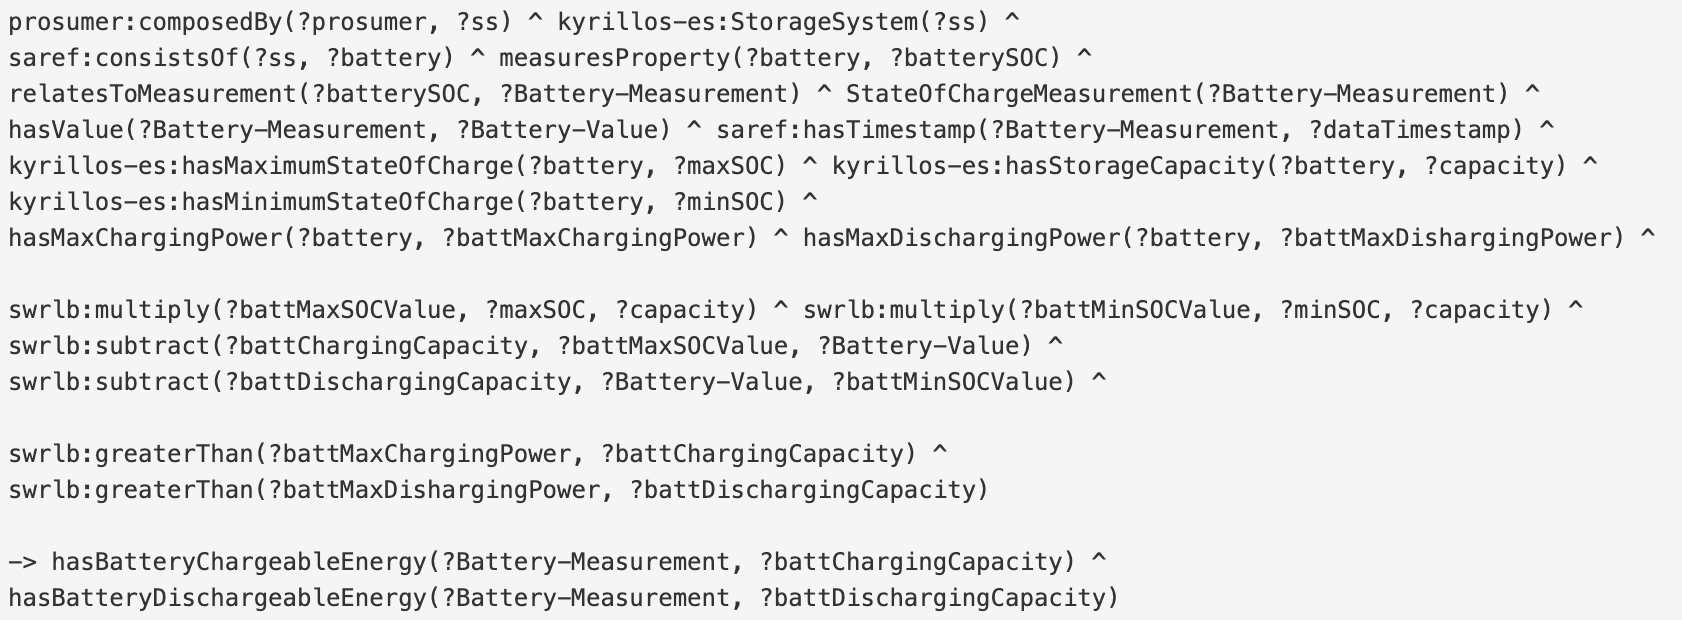
\includegraphics[width=15cm]{images/both >.png}
    \caption{Screenshot della quarta regola.}
    \label{fig:bothgreater}
\end{figure}

\section{SPARQL}
Nella seguente sezione verranno mostrate le query SPARQL e relativi risultati applicati agli individui creati nell'ontologia.

Si nota che per praticità, siccome sono query molto lunghe, verranno mostrate solamente parti delle query come screenshot e i risultati, mentre le query complete sono disponibili nei relativi file di testo che verranno mostrati.


\subsection{PREFIX}
Per leggibilità i prefissi utilizzati per le query SPARQL verranno visionati solamente in questa sezione, siccome ripetitivi per ogni query.

Si può quindi notare l'utilizzo in particolare dell'ontologia \textit{battery}, la nuova ontologia \textit{prosumer}, con anche \textit{SAREF} e \textit{Interconnect}.

\begin{figure}[H]
    \centering
    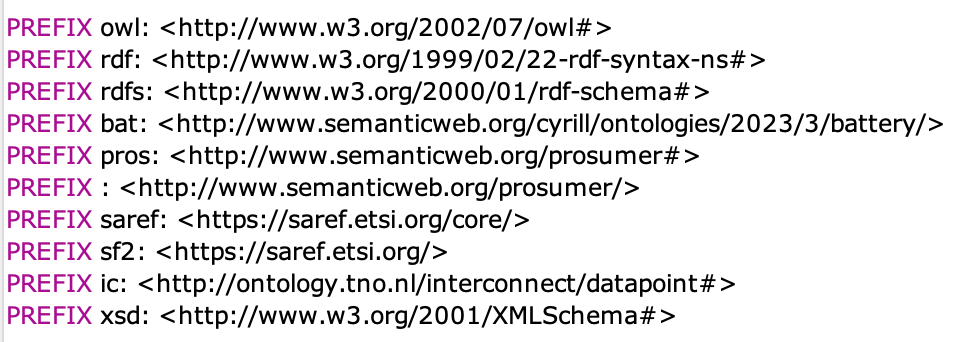
\includegraphics[width=15cm]{images/prefissi.png}
    \caption{Prefissi da anteporre alle query sull'ontologia.}
    \label{fig:prefix}
\end{figure}

\subsection{Query che calcola l'energia che può fornire o assorbire uno Storage System}

Dato uno Storage System composto da una o più batterie, si vuole calcolare l'energia che il sistema nel suo complesso può assorbire o fornire.

Per ogni batteria, c'è un valore che rappresenta l'energia presente in un dato timestamp, percìo si sommano i valori delle varie batterie presenti nello storage dello stesso timestamp.

\begin{figure}[H]
    \centering
    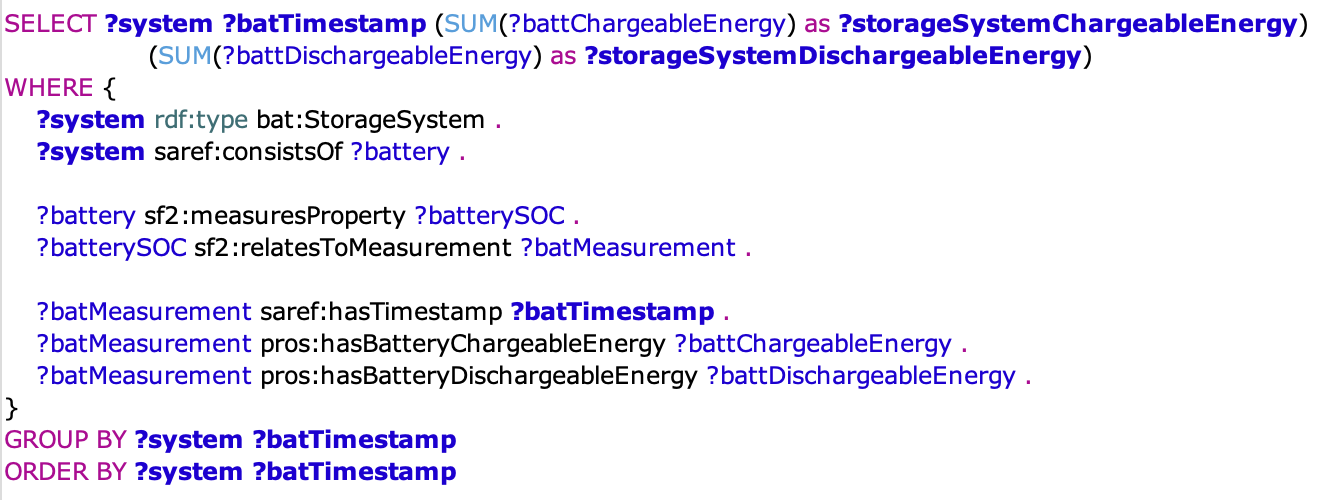
\includegraphics[width=15cm]{images/subquery.png}
    \caption{Query per il calcolo dell'energia che uno Storage System può assorbire o fornire.}
    \label{fig:subquery}
\end{figure}

La query è disponibile nella repository di \href{https://github.com/19eddie/SemanticWeb-Assignment02-03}{Github} nel file \href{https://github.com/19eddie/SemanticWeb-Assignment02-03/blob/main/SPARQL%20energia%20che%20pu%C3%B2%20assorbire%20o%20fornire%20uno%20StorageSystem.txt}{SPARQL energia che può assorbire o fornire uno StorageSystem.txt}

Dall'esecuzione della query otteniamo dunque la quantità di energia che ogni Storage System può assorbire e immettere nel relativo timestamp. \ref{fig:subquery_res}

\begin{figure}[H]
    \centering
    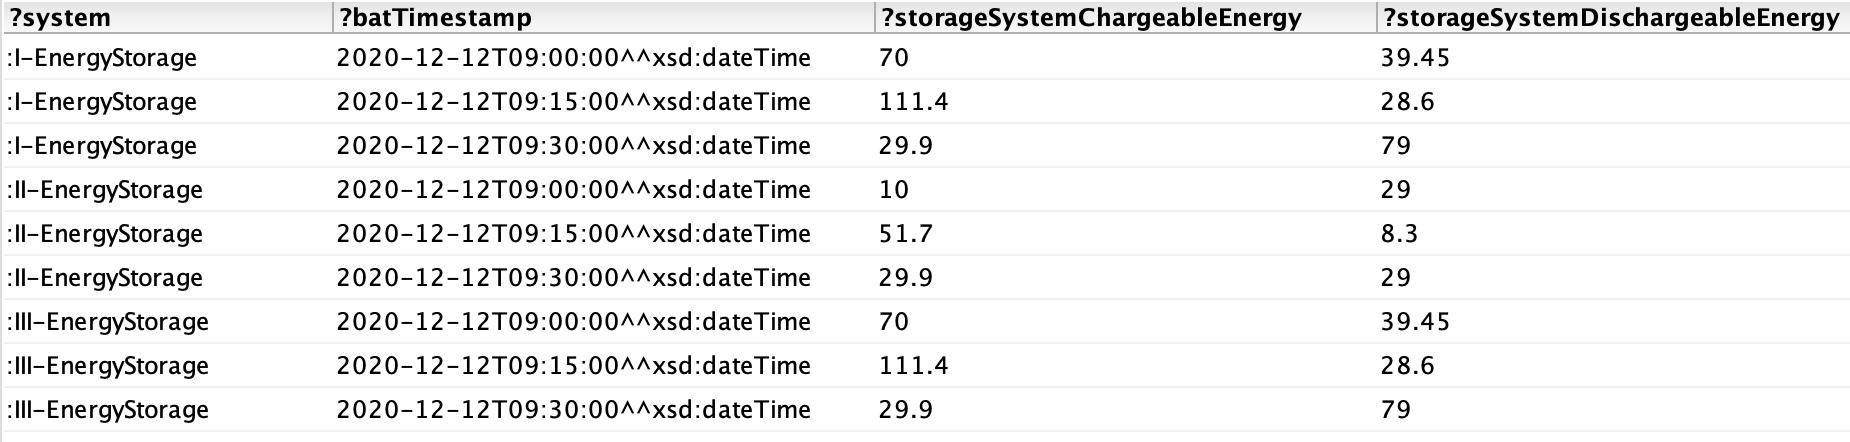
\includegraphics[width=15cm]{images/subquery_res.png}
    \caption{Risultati della query per il calcolo dell'energia che uno Storage System può assorbire o fornire.}
    \label{fig:subquery_res}
\end{figure}

\subsection{Query sul calcolo della flessibilità del contatore M1}



\subsection{Query per il calcolo di M1 e M2 in prosumer di configurazione 1 e 2}

\subsection{Query per il calcolo di M1, M2 e M3 in prosumer di configurazione 3}